\documentclass{beamer}

\usepackage{amsmath}
\usepackage{amssymb}
\usepackage{graphicx}

% Dresden
\usetheme{Dresden}

\begin{document}

	\title{A Simple Coarse-Grained Model of a Carbon Nanotube Forest Interacting with a Rigid Substrate}
	
	\author[Andrew Marmaduke]{Andrew Marmaduke\\{\small Advised by Dr. Golovaty and Dr. Wilber}}
	\institute{The University of Akron}
	\subject{Master Thesis}
	
	\frame{ \maketitle }

	\frame {
		\frametitle{Table of contents}
		\tableofcontents
	}

	\section{Motivation}

	\frame {
		\frametitle{Motivation}
		 A nanoscale mechanism of adhesion is believed to be governed by van der Waals interactions. Carbon nanotubes in particular have been suggested as a material for adhesive applications. Understanding the van der Waals interactions in the context of carbon nanotubes is crucial for potential use in applications.
	}
	
	\section{Model}

	\frame {
		\frametitle{Coarse-grained modeling}
		Coarse-grained modeling is a technique used to model materials, typically at a mesoscopic (between nano and micro) scale, with discrete objects. In comparison to molecular dynamics the time and length scales that are explored by coarse-grained techniques are larger.
	}
	
	\frame {
		\frametitle{Coarse-grained modeling of carbon nanotubes}
		\centering
		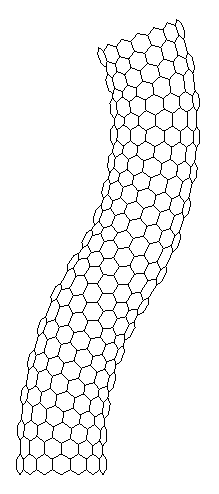
\includegraphics[scale=.20]{./fig/ch1/Nanotube.eps}
		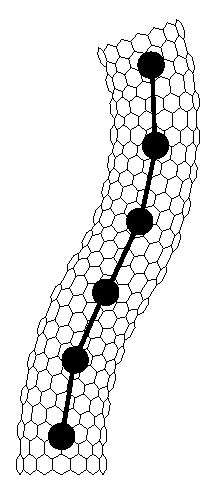
\includegraphics[scale=.20]{./fig/ch1/NanotubeParticle.eps}
		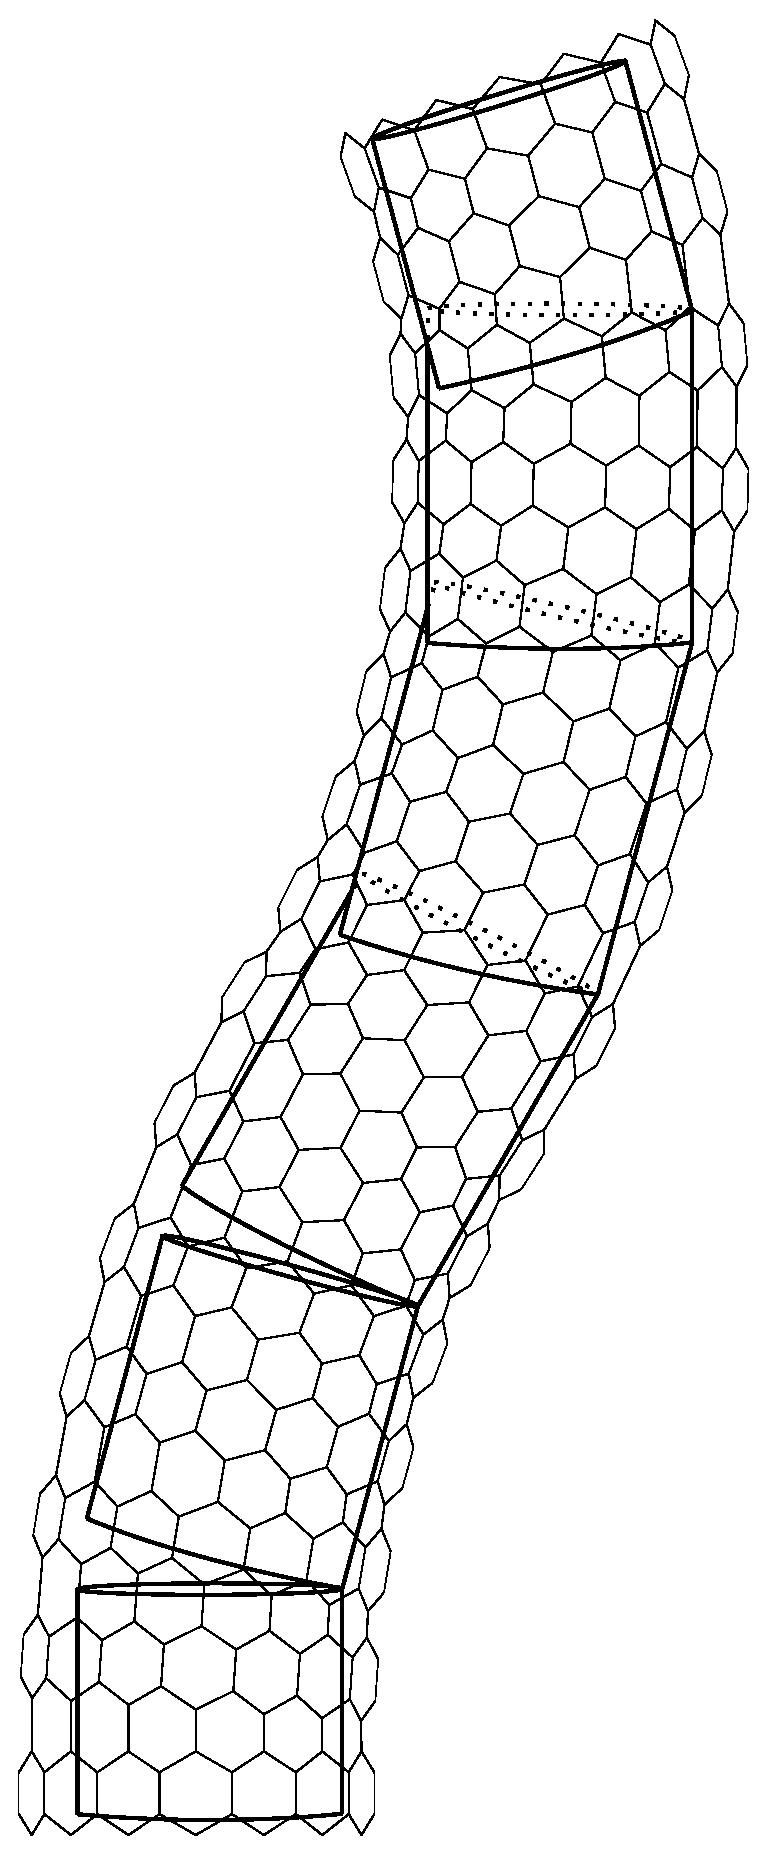
\includegraphics[scale=.20]{./fig/ch1/NanotubeCylinder.eps}
	}
	
	\frame {
		\frametitle{Geometry of carbon nanotube/substrate system}
		\input{./fig/ch2/geometry.eps_tex}
	}		
	
	\frame {
		\frametitle{Extensible and torsional springs}
		
		Extensible springs form bonds between adjacent particles of a fiber,
		\begin{equation*}
			E_e = \gamma \sum_{j=1}^m \sum_{i=1}^{n_j} \left[ \left( \|\Delta \textbf{r}_i^{(j)} \| - \ell \right)^2 \right].
		\end{equation*}
		
		Torsional springs between adjacent bonds keep particles of the fiber collinear,
		\begin{equation*}
			E_b = 2\beta \sum_{j=1}^m \sum_{i=1}^{n_j} \left[ \frac{\|\Delta \textbf{r}_i^{(j)} \| \|\Delta \textbf{r}_{i-1}^{(j)} \| - \Delta \textbf{r}_i^{(j)} \cdot \Delta \textbf{r}_{i-1}^{(j)}}{\|\Delta \textbf{r}_i^{(j)} \| \|\Delta \textbf{r}_{i-1}^{(j)} \| + \Delta \textbf{r}_i^{(j)} \cdot \Delta \textbf{r}_{i-1}^{(j)}} \right].
		\end{equation*}
	}
	
	\frame {
		\frametitle{Van der Waals interactions}
		
		Van der Waals interactions between pairs of particles is modeled by the shifted Lennard-Jones potential,

		\begin{equation*}
			U(x; \varepsilon, \sigma) = \varepsilon \left[ \left( \frac{\sigma}{x} \right)^{12} - 2 \left( \frac{\sigma}{x} \right)^6 \right],
		\end{equation*}
		
		\begin{equation*}
			U_c(x; \varepsilon, \sigma) = \left\{ 
				\begin{array}{lr}
					U(x; \varepsilon, \sigma) - U(r_c; \varepsilon, \sigma) - \frac{dU}{dx}\bigg|_{x = r_c}(x - r_c), & x \leq r_c\\
					0, & x > r_c
				\end{array}
				\right. 
		\end{equation*}
	}
		
	\frame {
		\frametitle{Van der Waals interactions}		
		The total contribution of van der Waals interactions is
		
		\begin{multline*}
			E_v = \sum_{j=1}^m \sum_{i=1}^{n_j} \bigg[ \sum_{(h,k) \in P(j,i)} U_c \left( \| \textbf{r}_i^{(j)} - \textbf{r}_k^{(h)} \|; \varepsilon, \sigma \right) \\ + \sum_{k=1}^{n_-} U_c \left( \| \textbf{r}_i^{(j)} - \textbf{r}_k^{(-)} \|; \varepsilon_-, \sigma \right) \\ + \sum_{k=1}^{n_+} U_c \left( \| \textbf{r}_i^{(j)} - \textbf{r}_k^{(+)} \|; \varepsilon_+, \sigma \right) \bigg].
		\end{multline*}
	}
	
	\frame {
		\frametitle{Total energy and system evolution}
		
		The total energy of the system is the sum of the previous energies and a load on the top substrate,		
		
		\begin{equation*}
			E = E_b + E_e + E_v + \lambda x_1^{(+)} - \mu y_1^{(+)}.
		\end{equation*}
		
		The system evolves by dissipation-dominated dynamics,		
		
		\begin{equation*} \label{eqn:system}
	 		\frac{d\textbf{r}_i^{(j)}}{dt} = -\nabla_{\textbf{r}_i^{(j)}}E,\ \ \ 1 \leq j \leq m,\  1 \leq i \leq n_j.
		\end{equation*}
	}
	
	\section{Numerical experiments}	
	
	\frame {
		\frametitle{Numerical experiments}	
		The model is explored in three separate numerical experiments.
		\begin{enumerate}
			\item {
				Find equilibrium configurations of a free standing fiber
			}
			\item {
				Find equilibrium configurations of a fiber under compression
			}
			\item {
				Find critical detachment load on the top substrate
			}
		\end{enumerate}		
	}
	
	\frame {
		\frametitle{Free standing experiment}
		\centering
		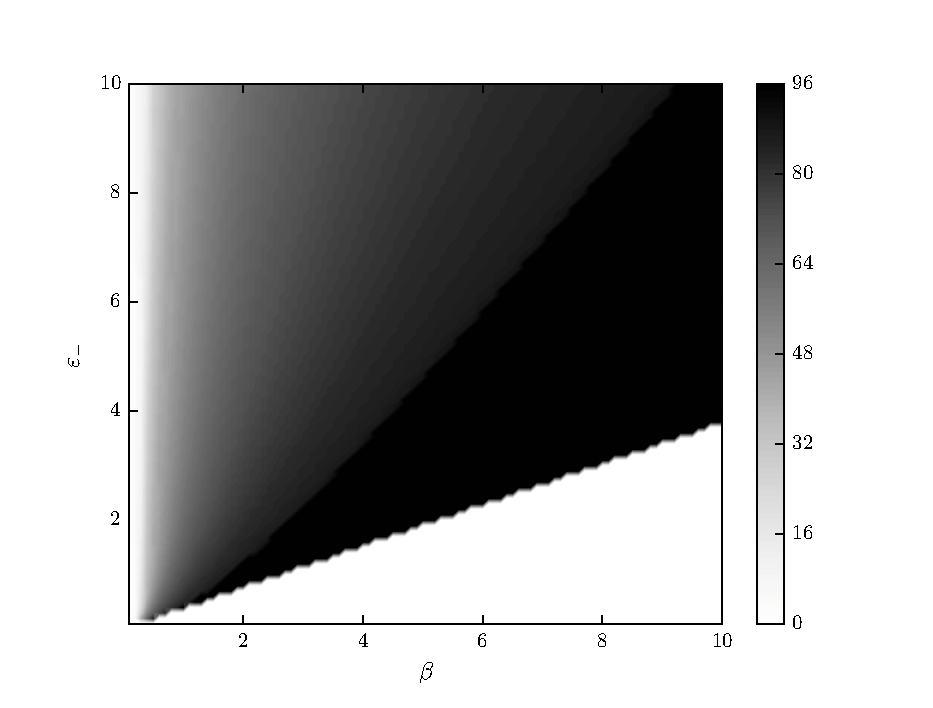
\includegraphics{./fig/ch3/fs/grid.eps}	
	}
	
	\frame {
		\frametitle{Free standing experiment}
		\centering
		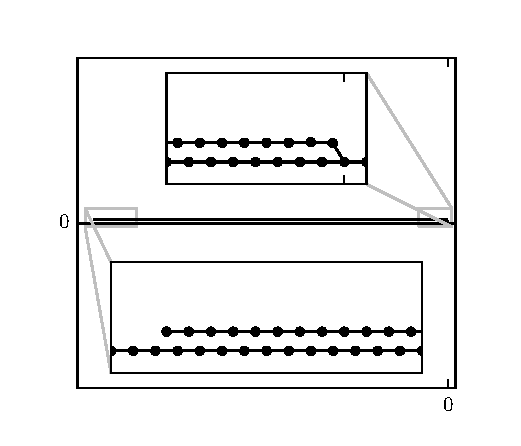
\includegraphics{./fig/ch3/fs/b5_eb3.eps}
	}		
	
	\frame {
		\frametitle{Free standing experiment}
		\centering
		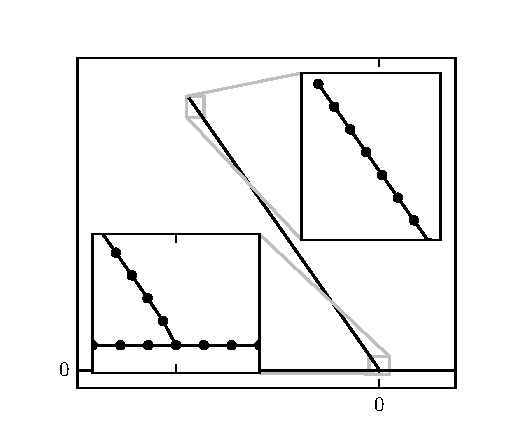
\includegraphics{./fig/ch3/fs/b10_eb3.eps}
	}		
	
	\frame {
		\frametitle{Free standing experiment}
		\centering
		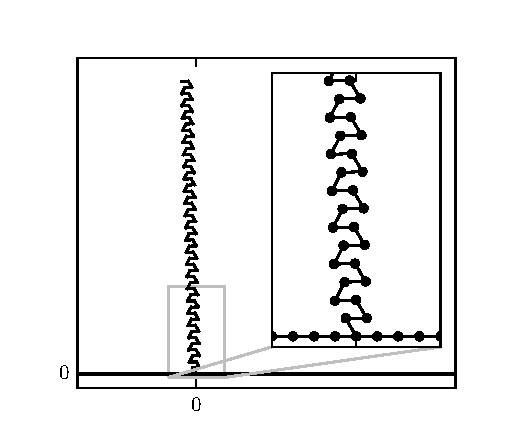
\includegraphics{./fig/ch3/fs/b0.1_eb3.eps}
	}
	
	\frame {
		\frametitle{Compression experiment}
		\centering
		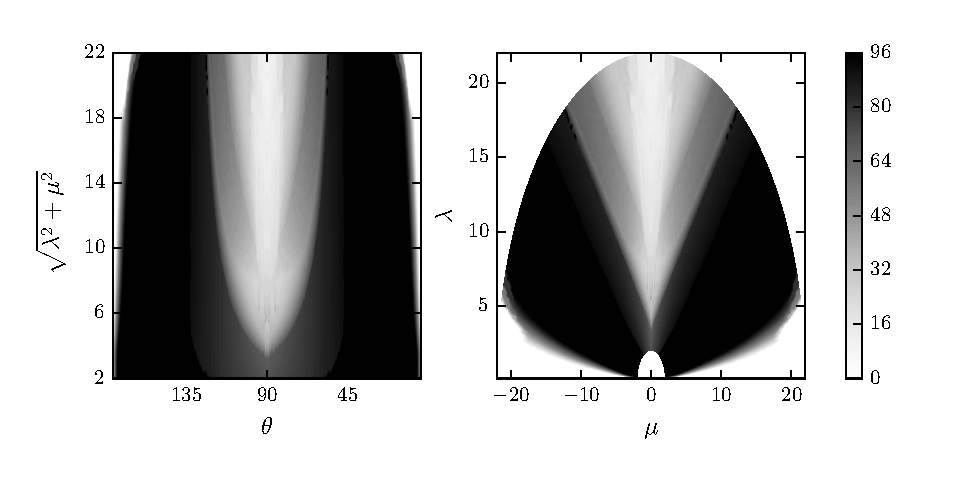
\includegraphics[scale=.75]{./fig/ch3/push/ref/grid.eps}
	}
	
	\frame {
		\frametitle{Compression experiment}
		\centering
		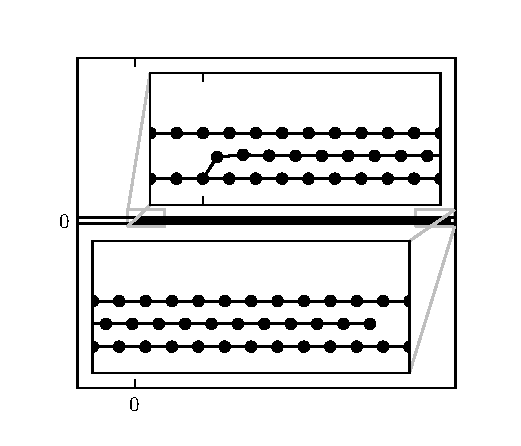
\includegraphics{./fig/ch3/push/ref/l5_m10.eps}
	}
	
	\frame {
		\frametitle{Compression experiment}
		\centering
		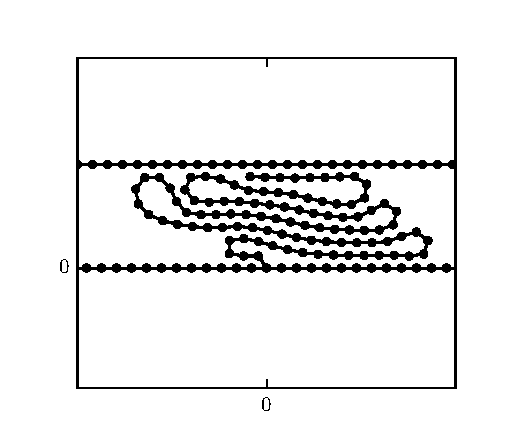
\includegraphics{./fig/ch3/push/ref/l19_m0.5.eps}
	}

	\frame {
		\frametitle{Compression experiment}
		\centering
		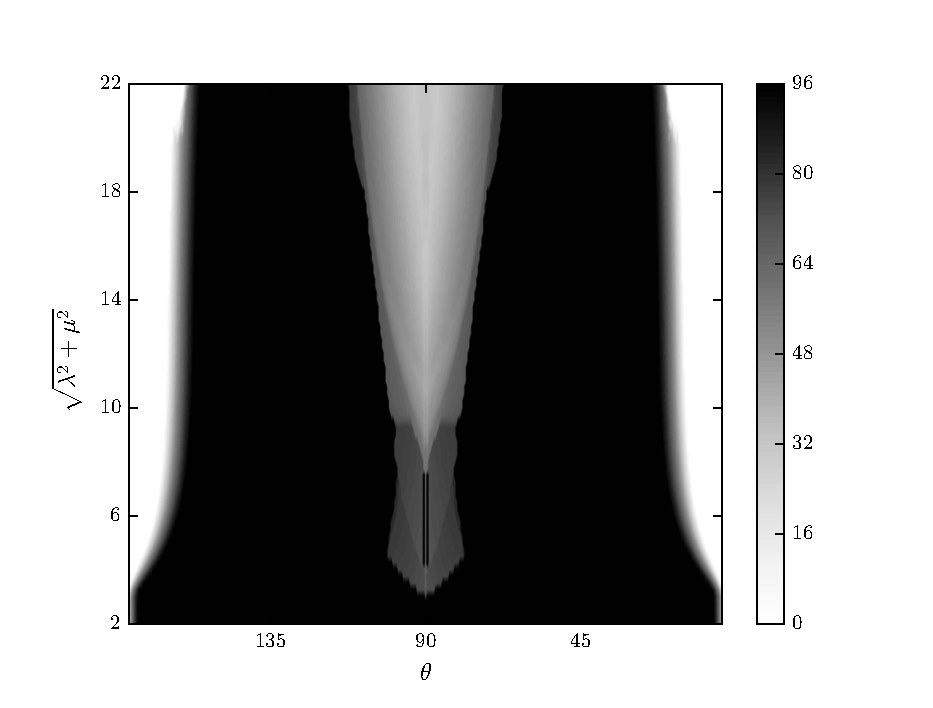
\includegraphics[scale=.75]{./fig/ch3/push/b100/grid.eps}
	}

	\frame {
		\frametitle{Compression experiment}
		\centering
		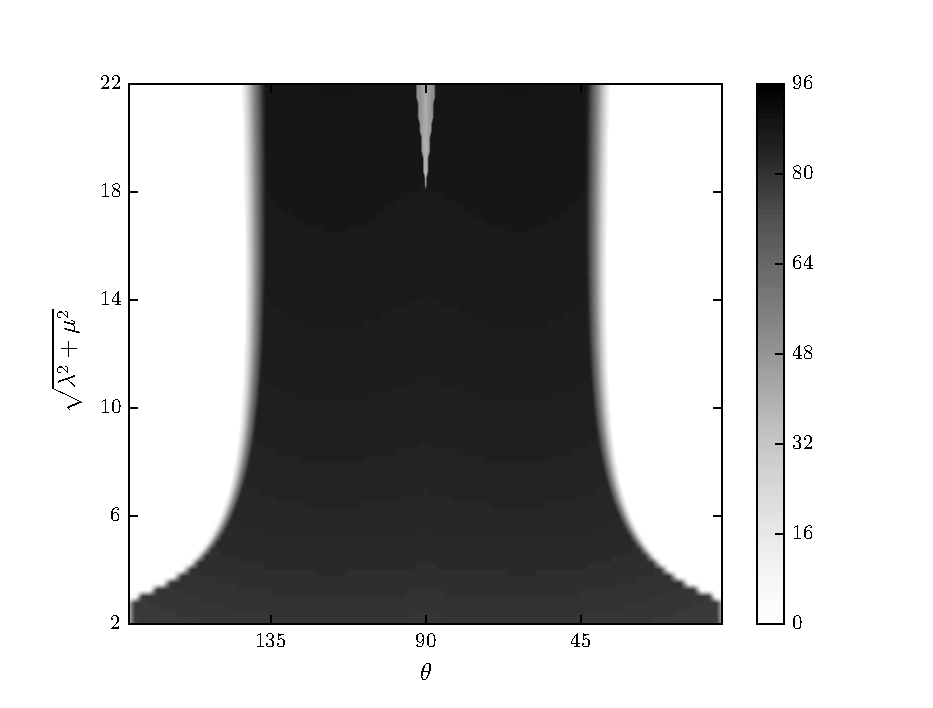
\includegraphics[scale=.75]{./fig/ch3/push/b1000/grid.eps}
	}

	\frame {
		\frametitle{Compression experiment}
		\centering
		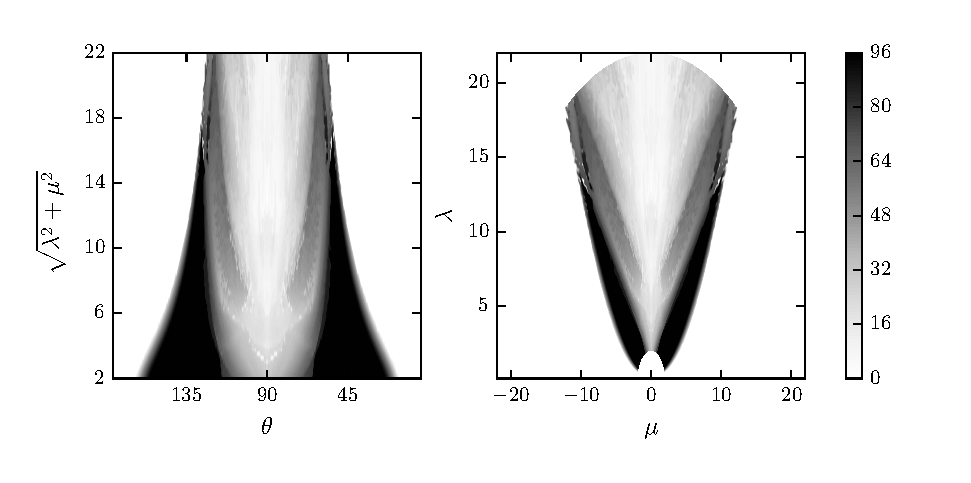
\includegraphics[scale=.75]{./fig/ch3/push/eb0.1_et0.1/grid.eps}
	}

	\frame {
		\frametitle{Detachment experiment}
		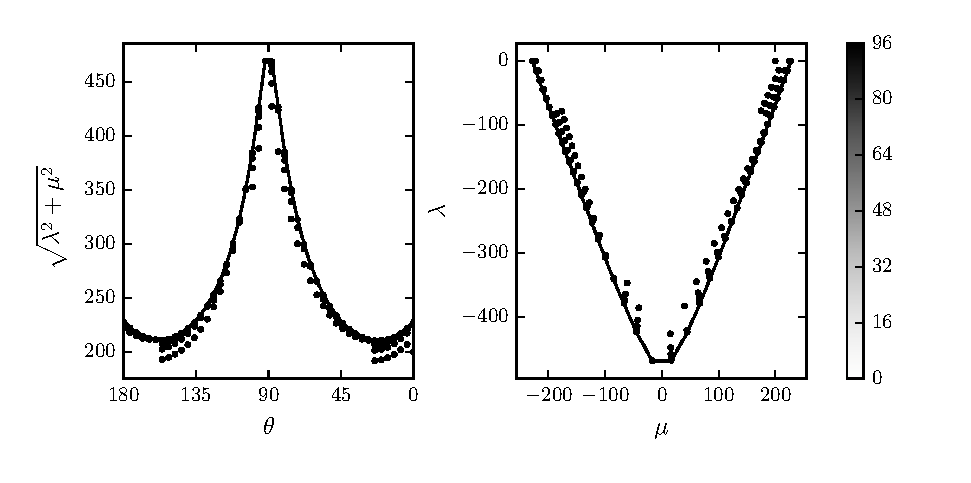
\includegraphics[scale=.75]{./fig/ch3/pull/ref/grid.eps}	
	}

	\frame {
		\frametitle{Detachment experiment}
		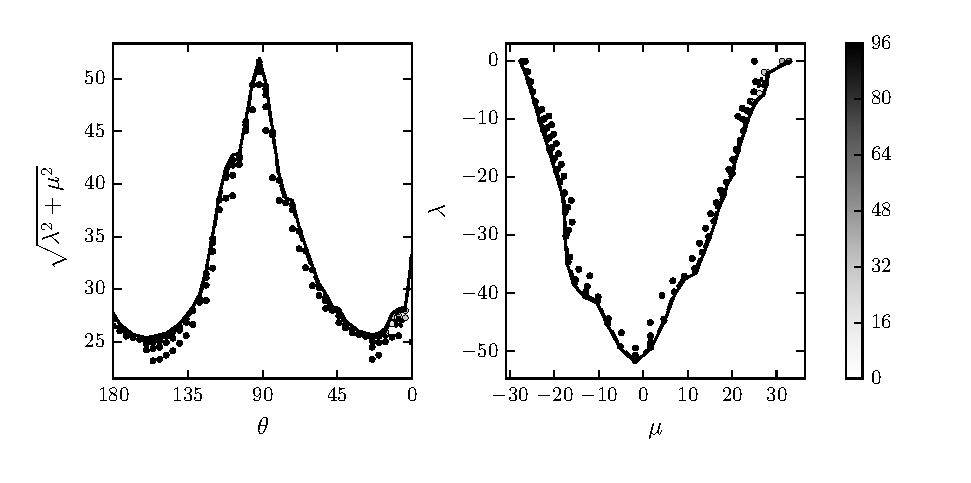
\includegraphics[scale=.75]{./fig/ch3/pull/eb0.1/grid.eps}
	}

	\frame {
		\frametitle{Detachment experiment}
		\centering
		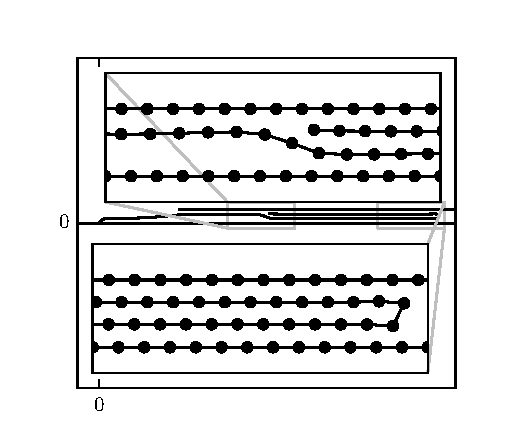
\includegraphics{./fig/ch3/pull/eb0.1/l0_m32.8.eps}
	}

	\frame {
		\frametitle{Detachment experiment}
		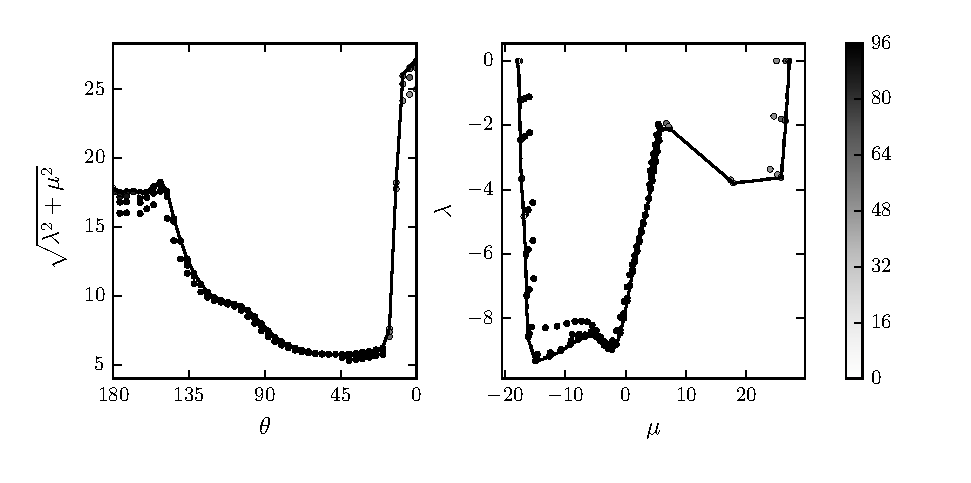
\includegraphics[scale=.75]{./fig/ch3/pull/eb0.01/grid.eps}
	}

	\frame {
		\frametitle{Detachment experiment}
		\centering
		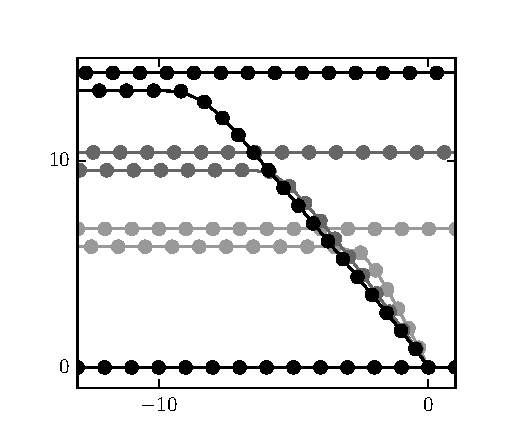
\includegraphics{./fig/ch3/pull/unzip_anim.eps}
	}

	\frame {
		\frametitle{Detachment experiment}
		\centering
		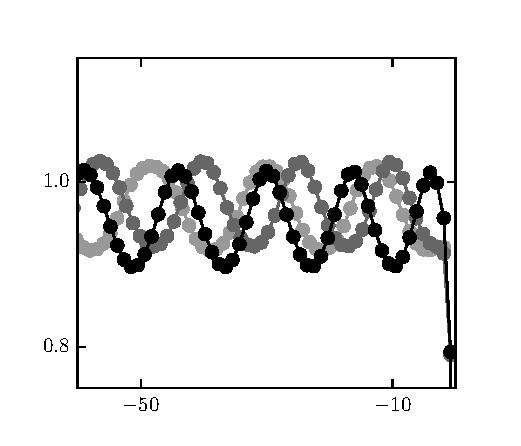
\includegraphics{./fig/ch3/pull/wave_anim.eps}
	}
	
	\frame {
		\frametitle{Compression experiment with ten fibers}
		\centering
		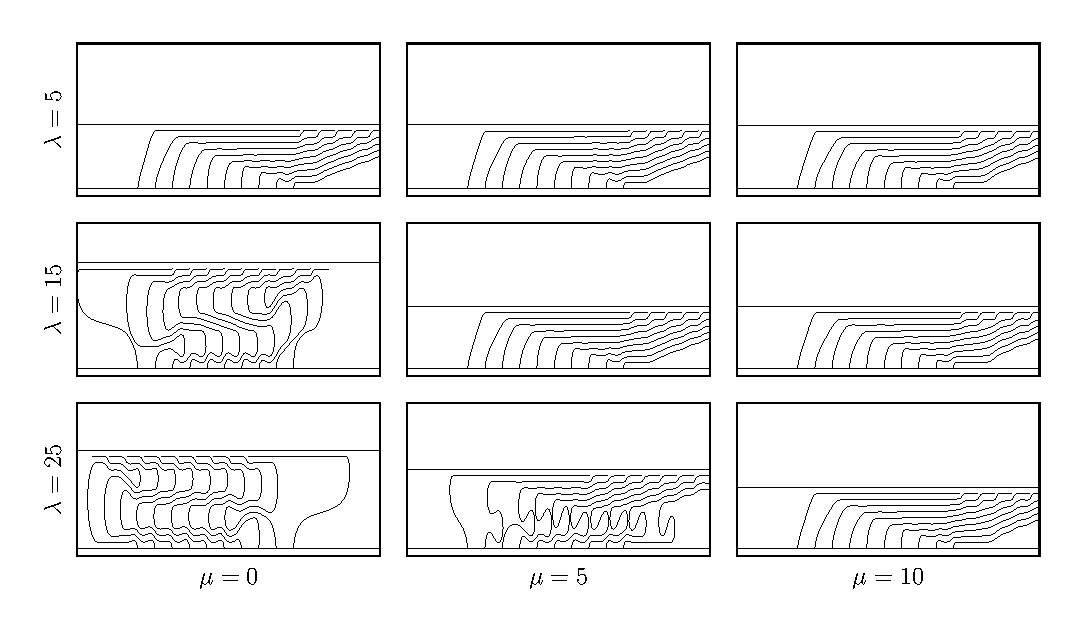
\includegraphics[scale=.5]{./fig/unequal.eps}	
	}
	
	\section{Conclusions}	
	
	\frame {
		\frametitle{Conclusions}
		We develop and simulate a simple coarse-grained model of adhesion motivated by carbon nanotubes. Linear relationships between model parameters in different experiments are discovered, in particular $\varepsilon_-$ and $\beta$ for the free-standing experiment and $\lambda$ and $\mu$ for the compression and detachment experiments. Equilibrium configurations qualitatively match those observed in experimental studies of carbon nanotubes forests and predictions continuum models of fiber adhesion.
	}


\end{document}
